\section{Beleuchtung \& Schattierung}

Eigenschaften eines Objektes:
\begin{itemize}
    \item Spiegelung
    \item Glanz / Matt
    \item Transparenz
    \item Glatt / Rau (Oberflächenstruktur)
    \item Farbe
    \item Struktur / Textur
    \item Brechnung des Lichts
    \item Anisotop (Richtungsabhängig)
\end{itemize}

\subsection{Energy}

\textit{Die Energy einer beleuchteten Fläche ist proportional zum Cosinus
zwischen Lichtrichtung und Flächennormale}\\

\textit{Fällt das Licht schräg auf die Fläche, muss eine grössere
Fläche mit Licht beleuchtet werden -> Fläche erscheint dünkler}

\subsection{Beleuchtungsmodelle}

\textit{Reale Beleuchtung ist seht aufwändig, daher wird einfacheres Modell verwendet.}

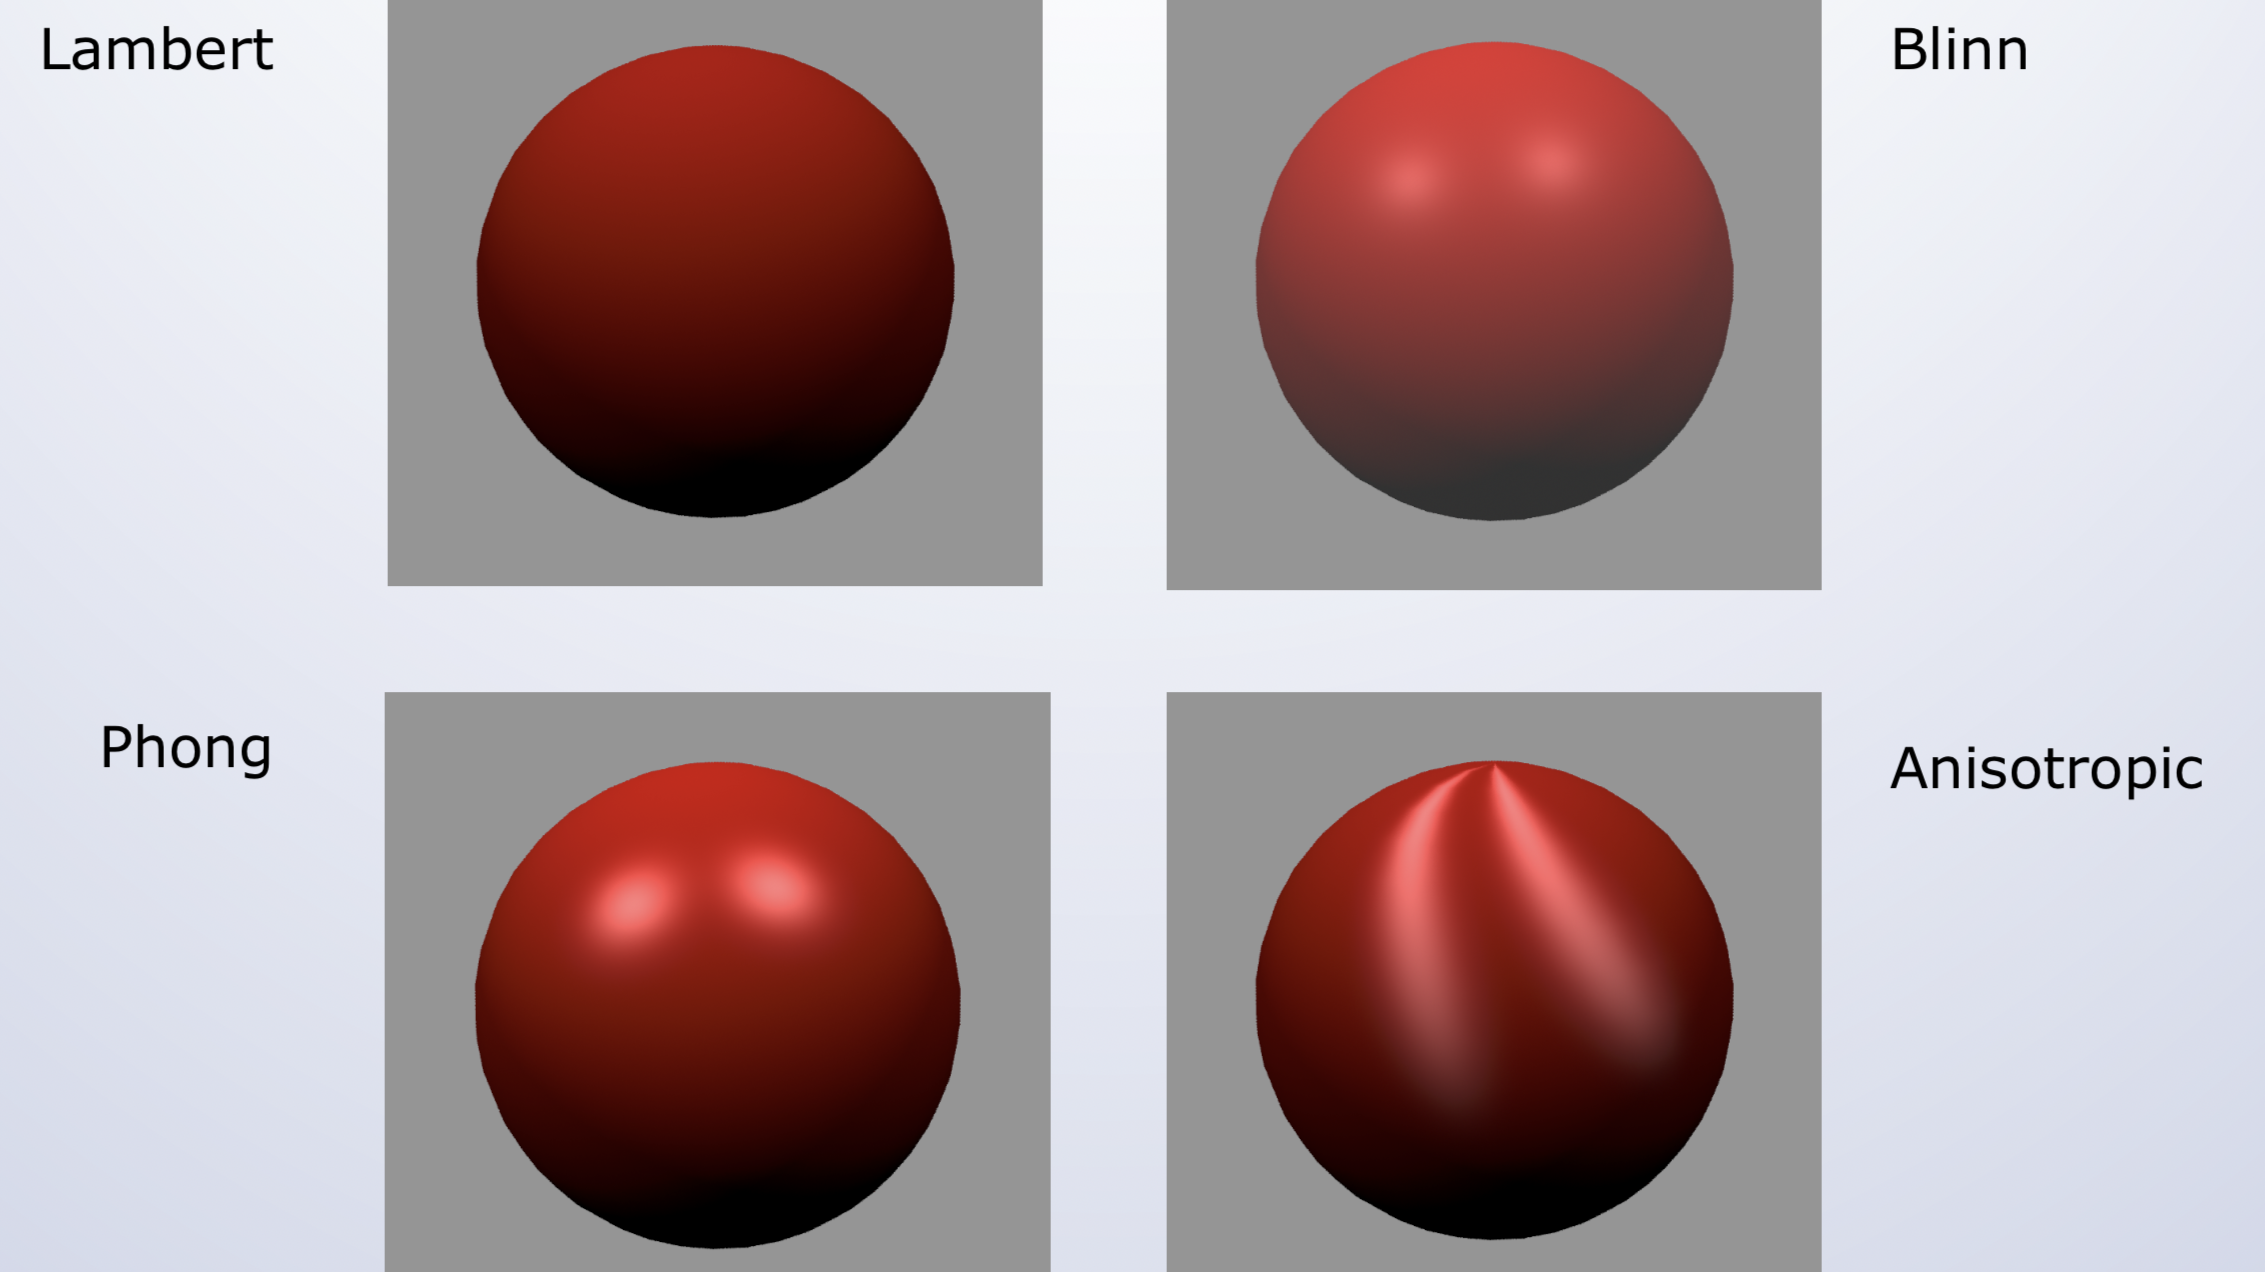
\includegraphics[width=0.45\textwidth]{assets/Beleuchtungsmodelle.png}

\subsubsection{Diffuse Reflektion (Lambert Modell)}

\begin{itemize}
    \item Gleichmässige Abstrahlung des Lichts in alle Richtungen
    \item Eigenschaften eines matten, nicht glänzenden Materials
    \item Schiefe Fläche = senkrechte Fläche / cos(a)
    \item reflektierte Intensität = Intensität der Lichtquelle * Reflektierungsfaktor * cosj \\
    \item cosj = Flächennormale(vektor) * Richtung zur Lichtquelle(vektor) \\
    \item Reflektierungsfaktor = Farbe des Materials
\end{itemize}

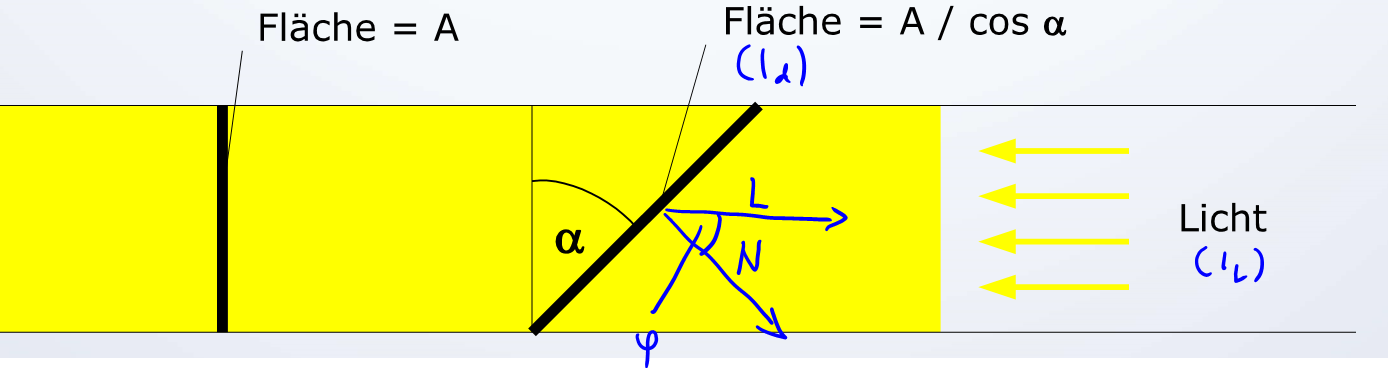
\includegraphics[width=0.5\textwidth]{assets/energy-model.png}\\

$I_d = I_L \cdot k_d \cdot \cos(\varphi)$ \\
$\cos(\varphi) = \vec{N} \cdot \vec{L}$ \\

$\vec{N}$: normalisiert Flächennormale \\
$\vec{L}$: Richtung zur Lichtquelle \\
$I_d$: reflektierte intensität \\
$I_L$: Intensität der Lichtquelle \\
$k_d$: Reflektionsfaktor \\

\subsubsection{Spiegelnde Reflektion (Phong Modell)}

\begin{itemize}
    \item[] Intensität Spiegelung = Intensität der Lichtquelle * Reflektierungsfaktor * cos\textsuperscript{n}(Winkel zwischen Betrachgung \& Reflektionsrichtung)
    \item[] n = Streuung des Lichts (hohes n -> Streuung nimmt schnell ab)
    \item[] Reflektierungsfaktor = Farbe der Reflektion
\end{itemize}

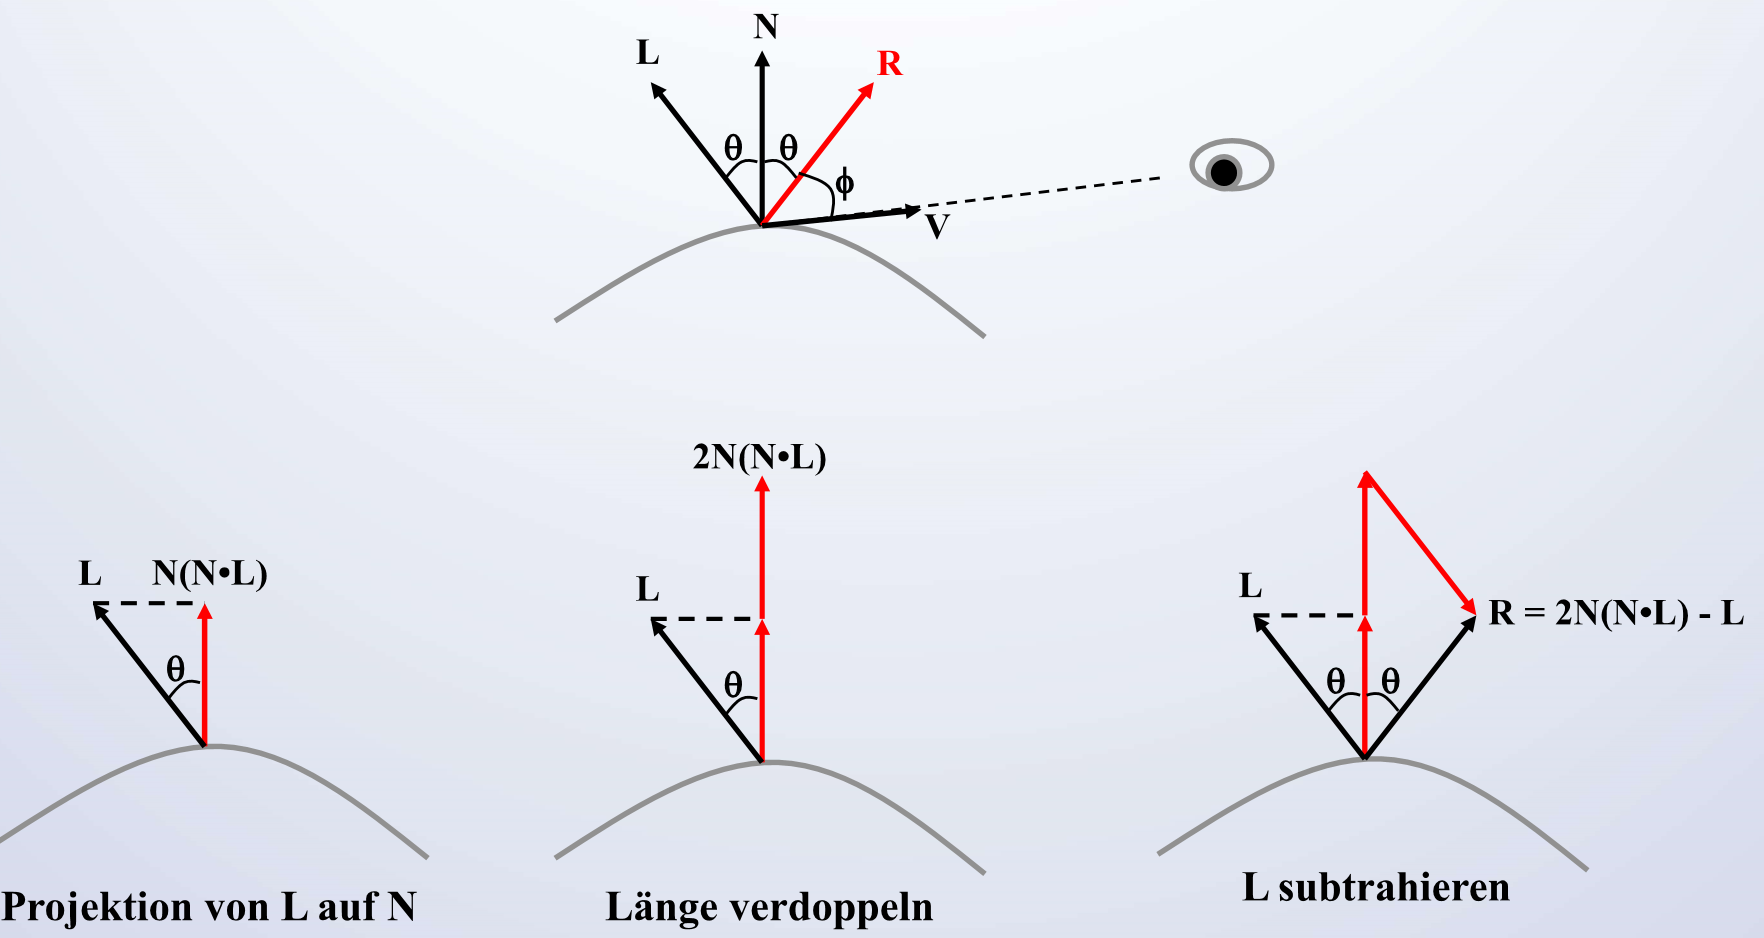
\includegraphics[width=0.5\textwidth]{assets/phong-modell.png}\\

$I_d = I_L \cdot k_d \cdot \cos(\phi)^{n_s}$ \\
$\cos(\phi) = \vec{V} \cdot \vec{L}$ \\
$R = 2\vec{N}(\vec{N} \cdot \vec{L}) - \vec{L}$ \\

$\vec{N}$: normalisiert Flächennormale \\
$\vec{L}$: Richtung zur Lichtquelle normalisiert \\
$I_d$: reflektierte intensität \\
$I_L$: Intensität der Lichtquelle \\
$k_d$: Reflektionsfaktor \\

\subsection{Scattering}

\textit{Licht wird teils auch reflektiert (gespiegelt)}

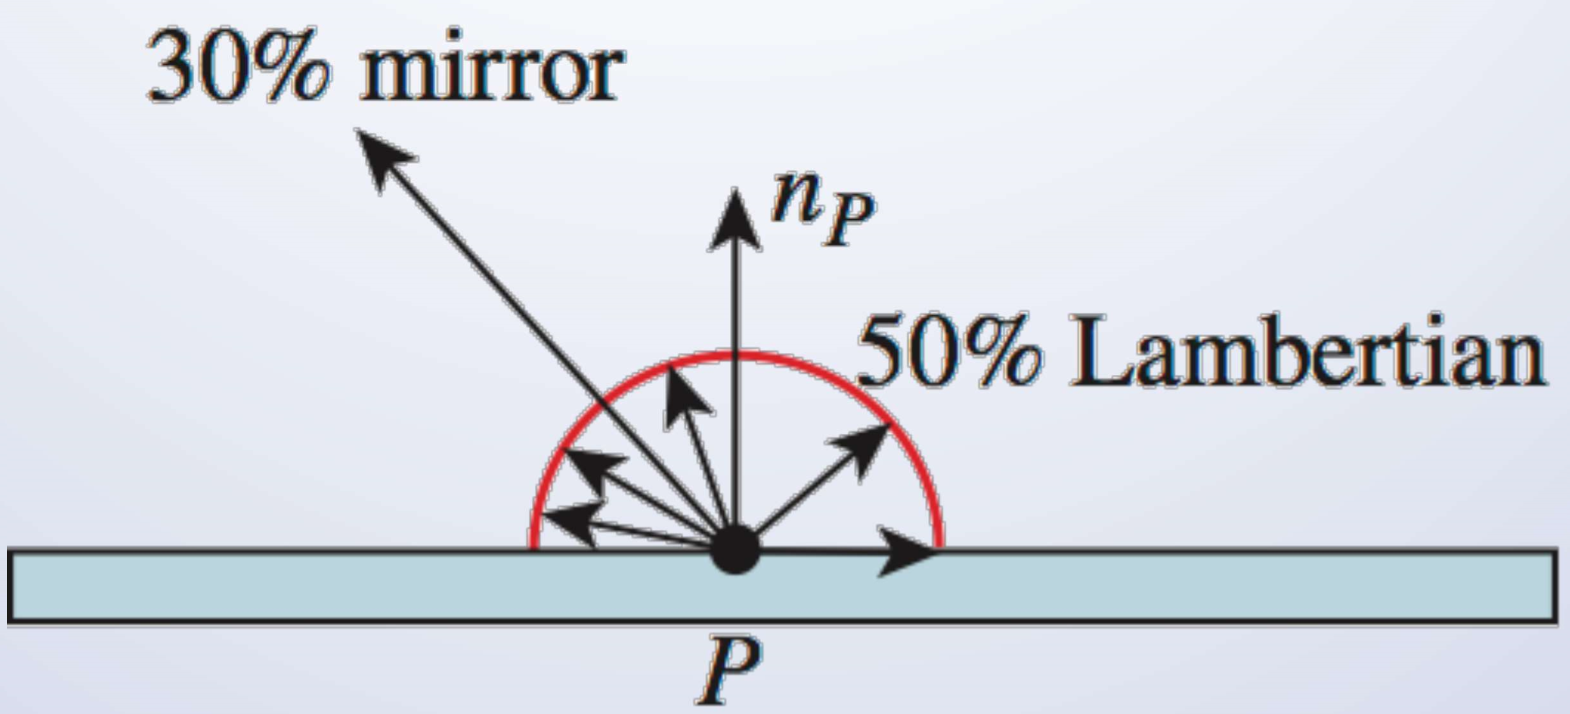
\includegraphics[width=0.35\textwidth]{assets/scattering-model.png}\\

\subsection{Farbe}

\textit{Reflektionskonstanten ($k_d$, $k_s$) hängen von der Wellenlänge ab.
    Diese werden beim einfachen Beleuchtungsmodell mit Konstanten für jeweils
    Rot Grün Blau definiert. Bsp: $k_s = (0.35,0.35,0.35)$, $k_d = (0.6,0,0)$.
}\\

\textit{$k_d$ : definiert die Farbe des Objektes}\\
\textit{$k_s$ : definiert die Farbe der Lichtquelle}

\subsection{Lichtabschwächung}

\textit{Lichtabschwächung nimmt mit dem Quadrat des Abstandes ab.
Jedoch zu schnell zu dunkel, daher beliebtes Modell:} \\

$f_{Att} = \frac{1}{(c_1 + c_2 d + c_3 d^2)}$ \\

$d$: Distanz
$c_n$: Konstanten

\subsection{Lichtquellen}

\begin{itemize}
    \item Ambiente Lichtquelle (Licht von überall)
    \item Direktionale Lichtquelle
    \item Punkt Lichtquelle
    \item Spot Lichtquelle (alles ausserhalb schwarz)
    \item Verteilte Lichtquelle (Licht mit Ausdehnung)
\end{itemize}

\subsection{Schattierung}

\begin{itemize}
    \item Konstanter Schattierung \\
    pro Fläche eine Beleuchtung (Farbe) berechnen

    \item Gouraud Schattierung \\
    Beleuchtung an den Ecken berechnen \\
    dazwischen interpolieren \\
    VertexShader

    \item Phong Schattierung \\
    Beleuchtungsberechnung pro Pixel \\
    FragmentShader
\end{itemize}